\chapter{Simulaci\'{o}n Computacional}

\section{Introducci\'{o}n}
Se estudia el cotransportador vSGLT mediante el servidor ANM (En ingl\'{e}s Anisotropic Network Model server) de la universidad de Pittsburg \cite{Eyal2015}\footnote{Recurso disponible en \url{http://anm.csb.pitt.edu/cgi-bin/anm2/anm2.cgi}}. El servidor ANM, como su nombre lo indica, es un servidor web el cual procesa la informaci\'{o}n de entrada del lado del cliente, en este caso, la informaci\'{o}n de entrada ser\'{a} el pdb y los par\'{a}metros de entrada para realizar los c\'{a}lculos del ANM, mientras que del lado del servidor se procesa la informaci\'{o}n suministrada v\'{i}a un c\'{o}digo escrito en C, el cual permite calcular los $n$ primeros modos normales, los factores b, las constantes el\'{a}sticas, las correlaciones entre distintas partes de la mol\'{e}cula y permite visualizar los modos de vibraci\'{o}n mediante java o pymol. En la FIGURA se encuentra un esquema de la entrada y salida de datos
\section{NMA previo de vSGLT}
Mediante el servidor ANM, en  aparece un estudio previo del simportador vSGLT, en el cual se utiliza un archivo de entrada que es el pdb de 3DH4 encontrado en la base de datos del Protein Data Bank. En este archivo no se determinan los residuos del la primera h\'{e}lice en cada subunidad. Aunque aparecen las posiciones de los residuos, el ANM server los ignora, haciendo el c\'{a}lculo \'{u}nicamente con los residuos conocidos.\\
Los c\'{a}lculos de salida mostrados son los factores b por cada n\'{u}mero de residuo y para cada distancia de corte $r_c$, variable entre $7\AA$ y $14\AA$. Ver figura \\ 
\begin{figure}
 \centering
  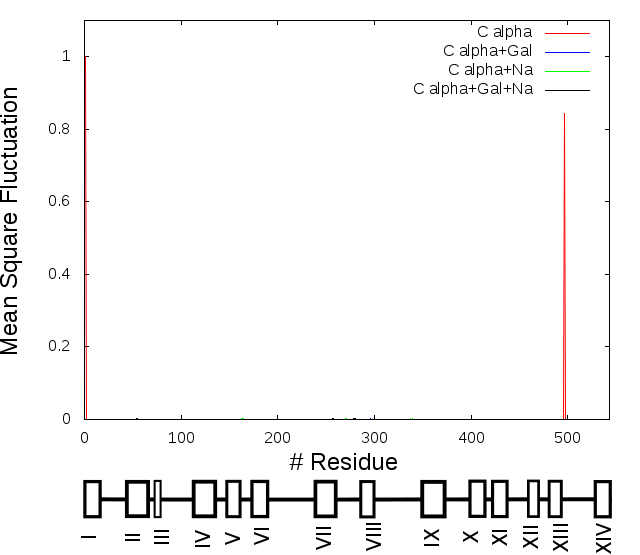
\includegraphics[scale=0.3]{./Kap4/ANM/ANM_server/grafica_7_A_n.png}
 %  \put(0,0){$R_c=7\AA$}
 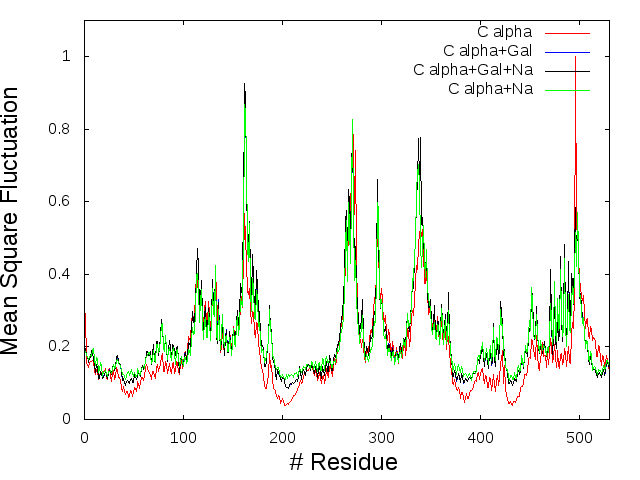
\includegraphics[scale=0.3]{./Kap4/ANM/ANM_server/grafica_8_A_n.png}
  %\put(0,0){$R_c=8\AA$}
  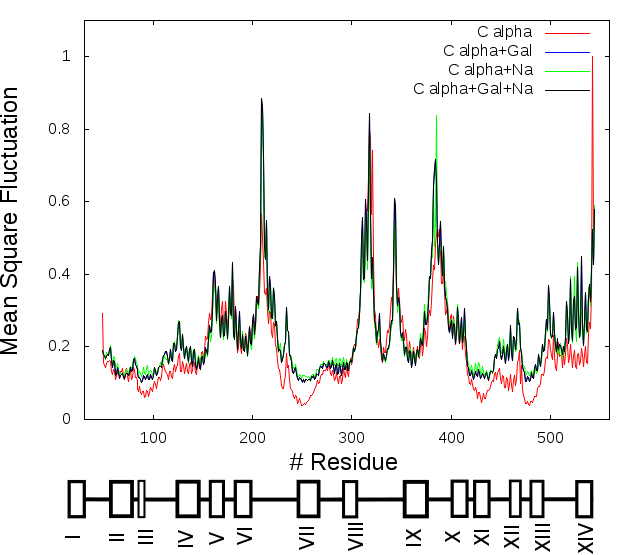
\includegraphics[scale=0.3]{./Kap4/ANM/ANM_server/grafica_9_A_n.png}
 % \put(0,0){$R_c=9\AA$}
   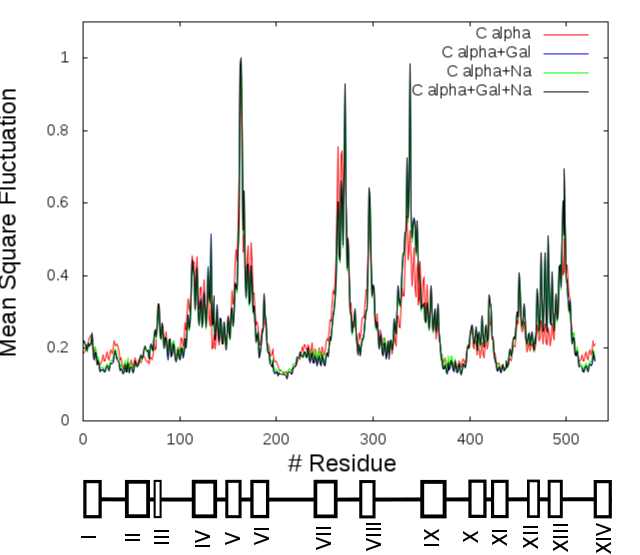
\includegraphics[scale=0.3]{./Kap4/ANM/ANM_server/grafica_10_A_n.png}
  % \put(0,0){$R_c=10\AA$}
    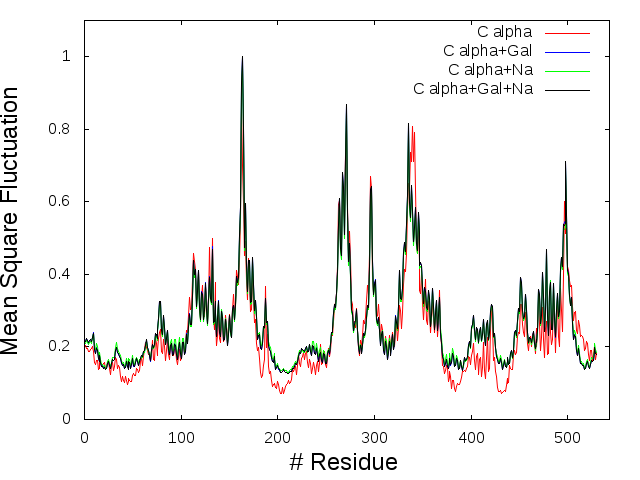
\includegraphics[scale=0.3]{./Kap4/ANM/ANM_server/grafica_11_A_n.png}
   % \put(0,0){$R_c=11\AA$}
     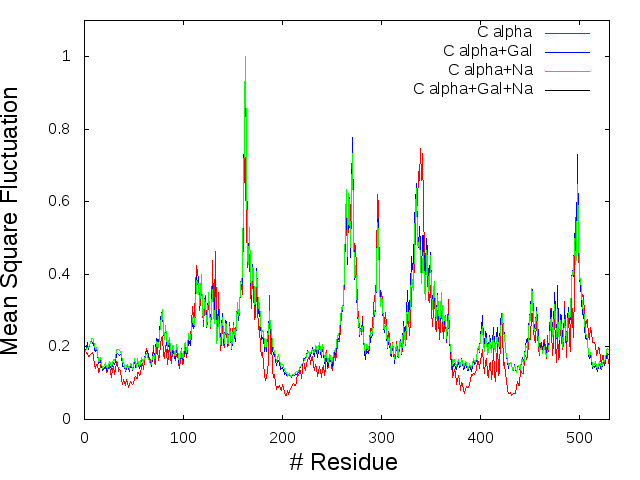
\includegraphics[scale=0.3]{./Kap4/ANM/ANM_server/grafica_12_A_n.png}
   %  \put(0,0){$R_c=12\AA$}
      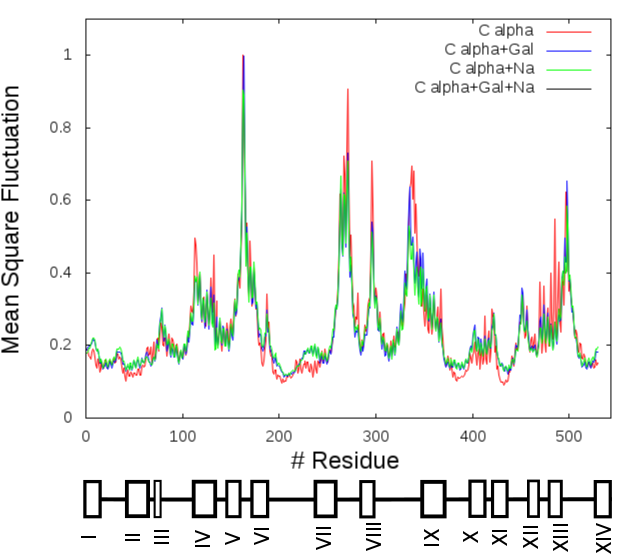
\includegraphics[scale=0.3]{./Kap4/ANM/ANM_server/grafica_13_A_n.png}
   %   \put(0,0){$R_c=13\AA$}
      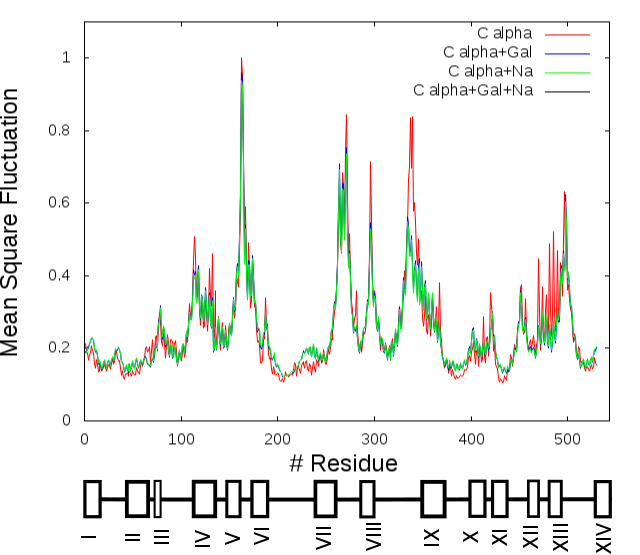
\includegraphics[scale=0.3]{./Kap4/ANM/ANM_server/grafica_14_A_n.png}
%\put(-50,-2){$R_c=14\AA$}
 \caption{Fluctuaciones ms normalizadas en funci\'{o}n del n\'{u}mero de residuo entre $7\AA\leq R_c\leq 14\AA$ usando  los primeros 100 modos. Los diferentes colores indican si la simulaci\'{o}n fue realizada sin el ion, el sustrato, con alguno de ellos o ambos.}
\end{figure}
\section{ANM para vSGLT}
\subsection{Preparaci\'{o}n del PDB}
Ya que en el mutante de vSGLT en la posici\'{o}n A294A, llamado 2XQ2 aparece resuelta la estructura cristalina del TM1 perteneciente a la cadena A, se usa el programa PyMol, y como archivos de entrada los pdbs 3DH4 y el de su mutante 2XQ2, para usar un archivo que sea cercano a la estructura real objeto de estudio, esto es, al cotransportador vSGLT.
\subsection{Resultados}
\begin{figure}
 \centering
  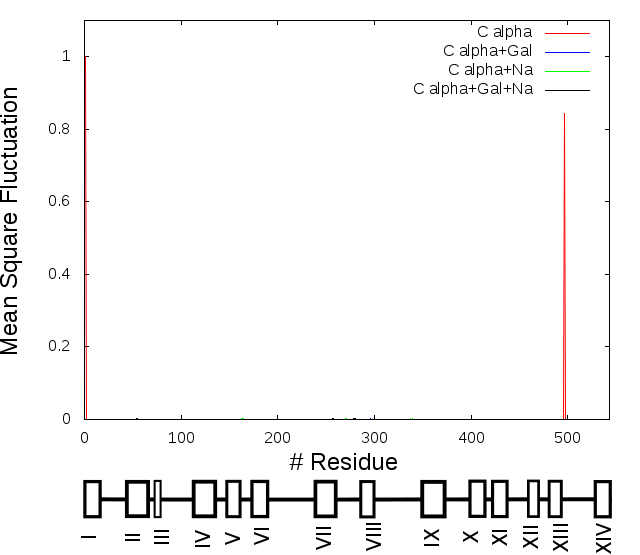
\includegraphics[scale=0.3]{./Kap4/ANM/ANM_server/grafica_7_A_n.png}
 %  \put(0,0){$R_c=7\AA$}
 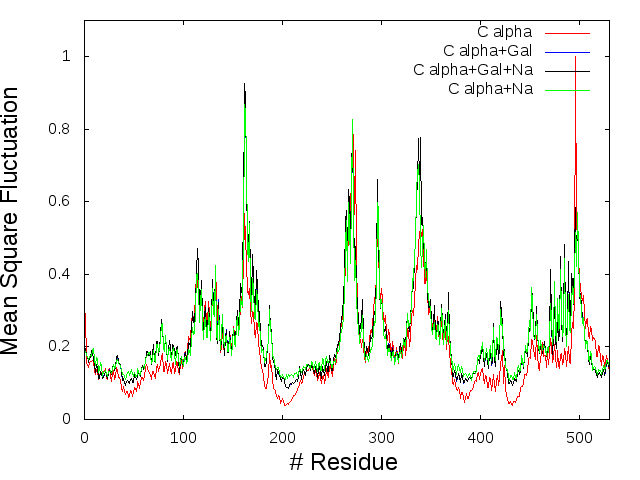
\includegraphics[scale=0.3]{./Kap4/ANM/ANM_server/grafica_8_A_n.png}
  %\put(0,0){$R_c=8\AA$}
  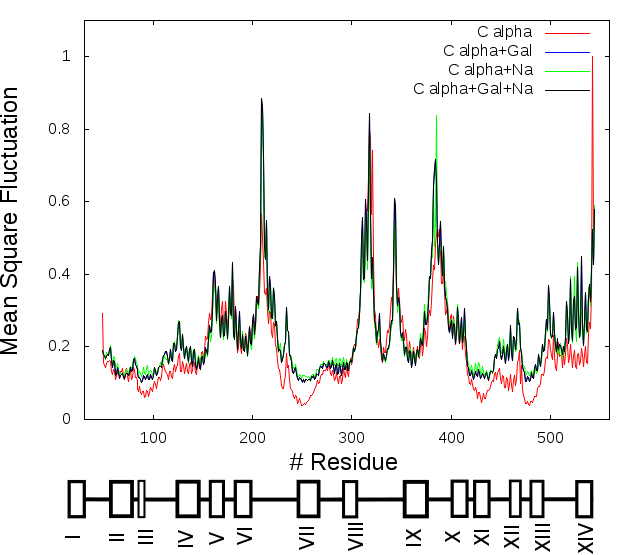
\includegraphics[scale=0.3]{./Kap4/ANM/ANM_server/grafica_9_A_n.png}
 % \put(0,0){$R_c=9\AA$}
   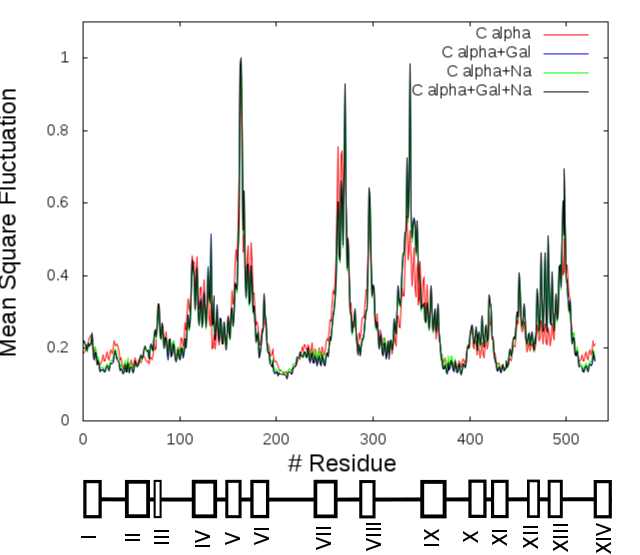
\includegraphics[scale=0.3]{./Kap4/ANM/ANM_server/grafica_10_A_n.png}
  % \put(0,0){$R_c=10\AA$}
    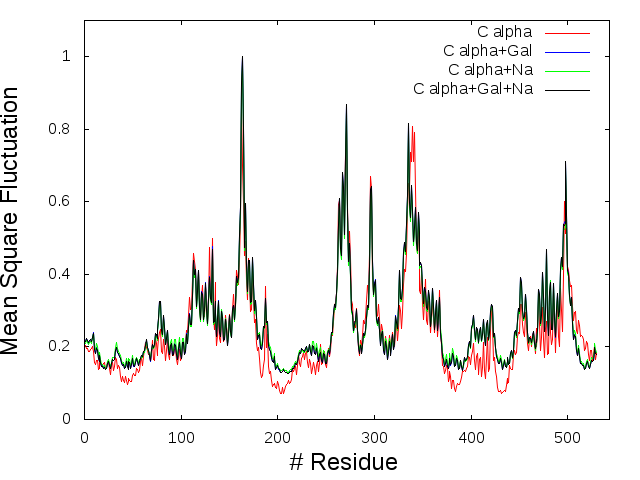
\includegraphics[scale=0.3]{./Kap4/ANM/ANM_server/grafica_11_A_n.png}
   % \put(0,0){$R_c=11\AA$}
     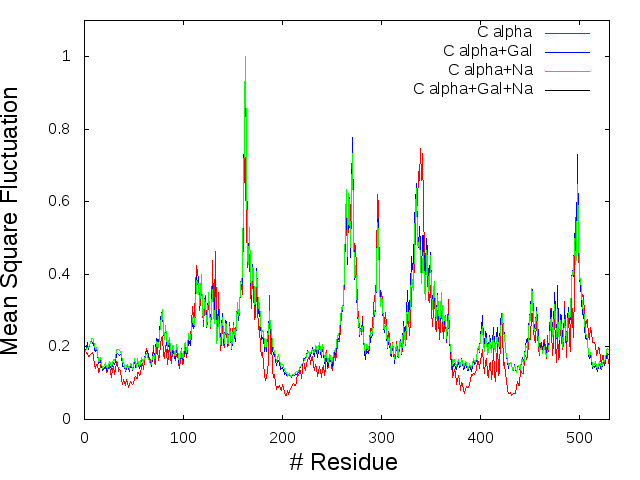
\includegraphics[scale=0.3]{./Kap4/ANM/ANM_server/grafica_12_A_n.png}
   %  \put(0,0){$R_c=12\AA$}
      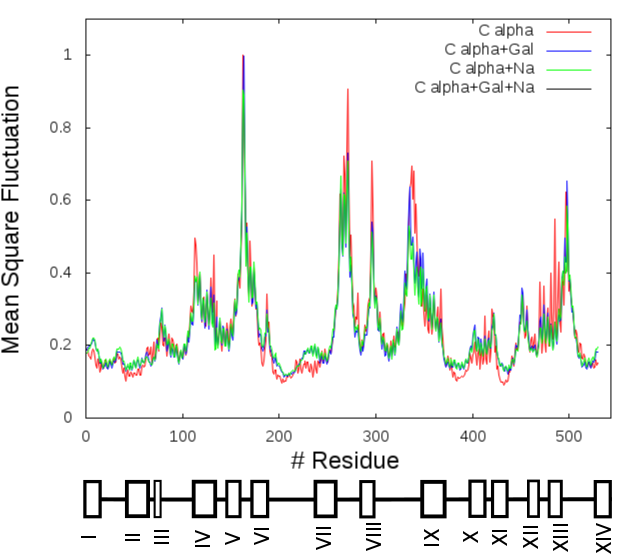
\includegraphics[scale=0.3]{./Kap4/ANM/ANM_server/grafica_13_A_n.png}
   %   \put(0,0){$R_c=13\AA$}
      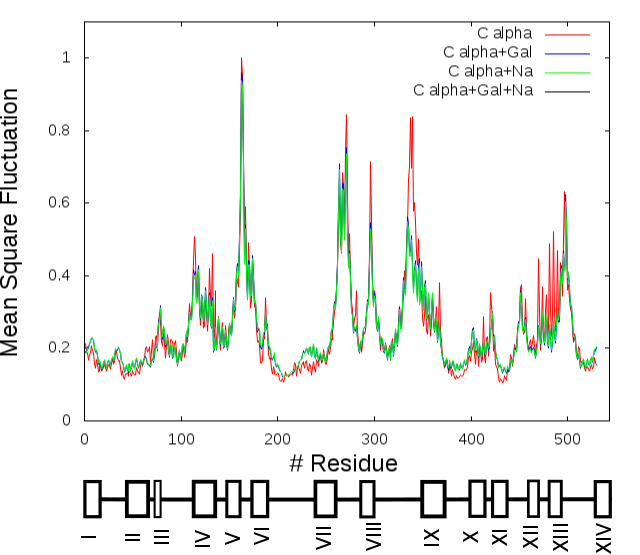
\includegraphics[scale=0.3]{./Kap4/ANM/ANM_server/grafica_14_A_n.png}
%\put(-50,-2){$R_c=14\AA$}
 \caption{Fluctuaciones ms normalizadas en funci\'{o}n del n\'{u}mero de residuo entre $7\AA\leq R_c\leq 14\AA$ usando  los primeros 100 modos. Los diferentes colores indican si la simulaci\'{o}n fue realizada sin el ion, el sustrato, con alguno de ellos o ambos.}
\end{figure}
\section{Modelo GNM de vSGLT}

\section{Mutante K294A de vSGLT con C-$\alpha$}